\documentclass[a4paper, 11pt]{article}
\usepackage[utf8]{inputenc}
\usepackage{graphicx}
\usepackage{subfig}
\usepackage{float}
\usepackage[export]{adjustbox}
\usepackage{float,gensymb,pdfpages}
\usepackage{marvosym,amsmath}
\usepackage{physics,amsfonts}
\usepackage{indentfirst}
\usepackage{gensymb}
\usepackage{comment} % enables the use of multi-line comments (\ifx \fi)  
\usepackage{fullpage} % changes the margin
\usepackage{tikz}
\usepackage[T1]{fontenc}
\usepackage[danish]{babel}
\usepackage{mathtools}
\usepackage{verbatim}

\newcommand{\B}[1]{\boldsymbol{#1}}
\newcommand{\batmanPic}[1]{
    \begin{tikzpicture}[baseline=0em, scale=#1]
        \draw[fill,black]   (-0.25,1.48) .. controls (-0.1,1.5) and (0.1,1.5) .. (0.25,1.48) -- (0.35,1.92) .. controls (0.425,1.8) and (0.41,1.3) .. (0.45,1.2) .. controls (0.6,1.05) and (1.96,1.05) .. (1.98,2.08) -- (5.93,2.08) .. controls (4.2,1.45) and (4,0.3) .. (4.2,-0.28) .. controls (2.4,-0.09) and (0.4,-0.5) .. (0,-2.052) .. controls (-0.4,-0.5) and (-2.4,-0.09) .. (-4.2,-0.28) .. controls (-4,0.3) and (-4.2,1.45) .. (-5.93,2.08) -- (-1.98,2.08) .. controls (-1.96,1.05) and (-0.6,1.05) .. (-0.45,1.2) .. controls (-0.41,1.3) and (-0.425,1.8) .. (-0.35,1.92) -- (-0.25,1.48);
    \end{tikzpicture}
} % End of \batman command

\newcommand{\batman}{\batmanPic{0.75}}
\begin{document}
\large\textbf{Numerical Solution of Ordinary Differential Equations} \hfill \textbf{Noah Huffman}
\par \normalsize Ph 20.3

\section{Motion of a mass on a spring}

\par First, Here are some plots of my numerical time evolutions of the system. Note that $X_{0}=0$, $V_{0}=0$ is an uninteresting initial condition because the system has not initial energy to make it dynamic.

 \begin{figure}[H]
\subfloat[$X_{0}=0$, $V_{0}=1$]{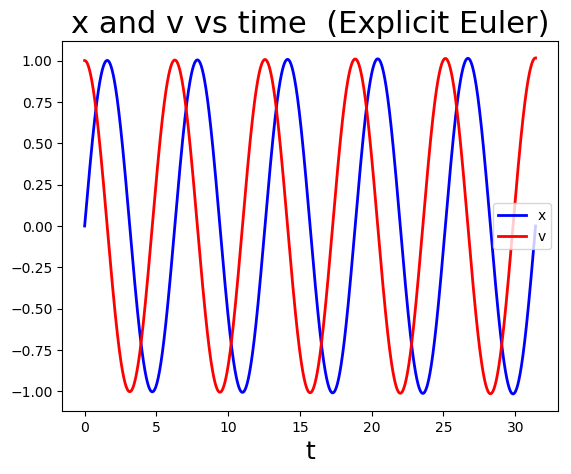
\includegraphics[width = 3in]{Explicit_X0_0_0_V0_1_0.png}} 
\subfloat[$X_{0}=1$, $V_{0}=0$]{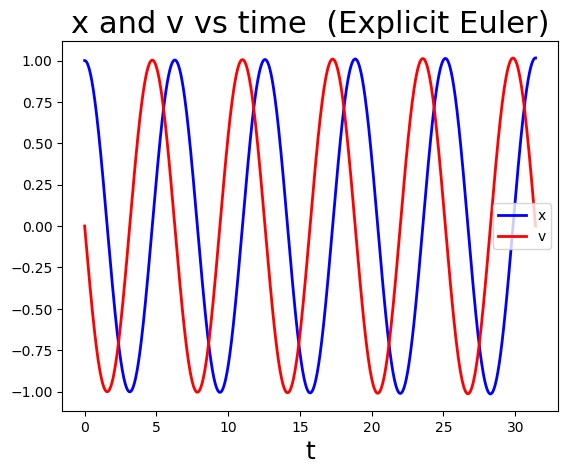
\includegraphics[width = 3in]{Explicit_X0_1_0_V0_0_0}}\\
\subfloat[$X_{0}=1$, $V_{0}=1$]{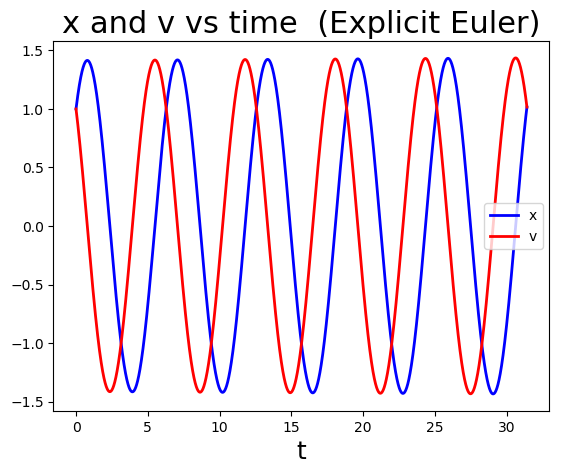
\includegraphics[width = 3in]{Explicit_X0_1_0_V0_1_0}}
\subfloat[$X_{0}=2$, $V_{0}=1$]{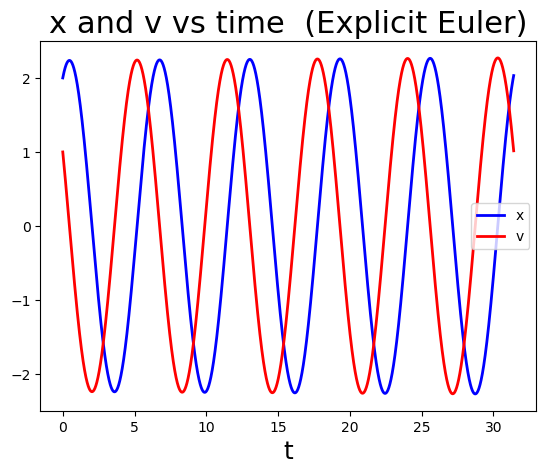
\includegraphics[width = 3in]{Explicit_X0_2_0_V0_1_0}} 
\caption{Explicit Euler numerical evolution of system over time for several initial conditions.}
\end{figure}

 \begin{figure}[H]
\subfloat[$X_{0}=0$, $V_{0}=1$]{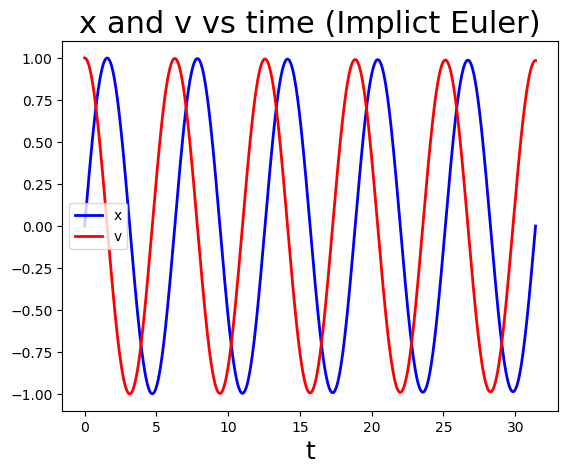
\includegraphics[width = 3in]{Implicit_X0_0_0_V0_1_0}} 
\subfloat[$X_{0}=1$, $V_{0}=0$]{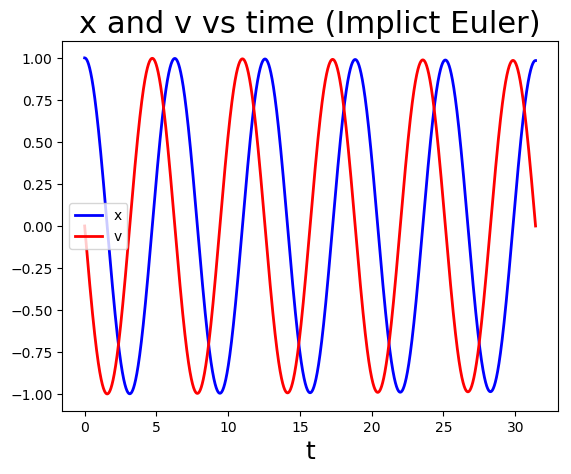
\includegraphics[width = 3in]{Implicit_X0_1_0_V0_0_0}}\\
\subfloat[$X_{0}=1$, $V_{0}=1$]{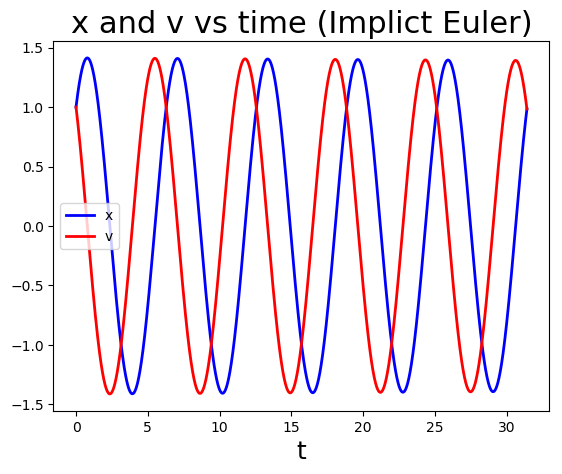
\includegraphics[width = 3in]{Implicit_X0_1_0_V0_1_0}}
\subfloat[$X_{0}=2$, $V_{0}=1$]{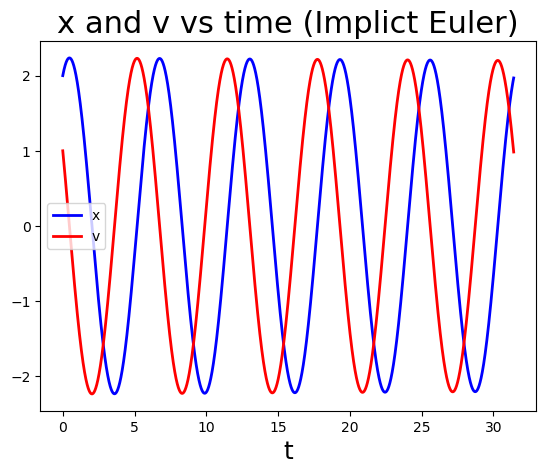
\includegraphics[width = 3in]{Implicit_X0_2_0_V0_1_0}} 
\caption{Implicit Euler numerical evolution of system over time for same initial conditions.}
\end{figure}

\section{Global errors}

 \begin{figure}[H]
\subfloat[$X_{0}=0$, $V_{0}=1$]{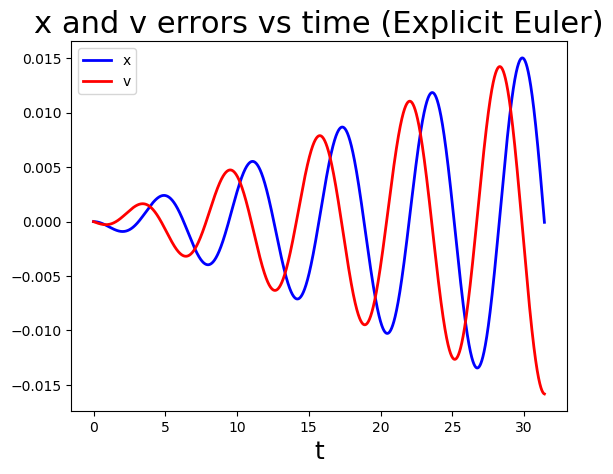
\includegraphics[width = 3in]{Explicit_Errors_X0_0_0_V0_1_0}} 
\subfloat[$X_{0}=1$, $V_{0}=0$]{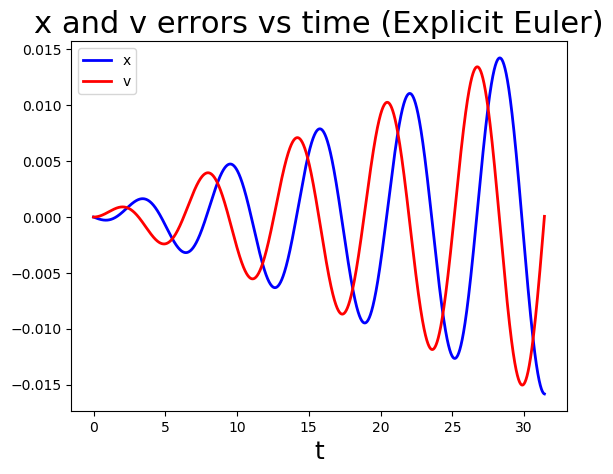
\includegraphics[width = 3in]{Explicit_Errors_X0_1_0_V0_0_0}}\\
\subfloat[$X_{0}=1$, $V_{0}=1$]{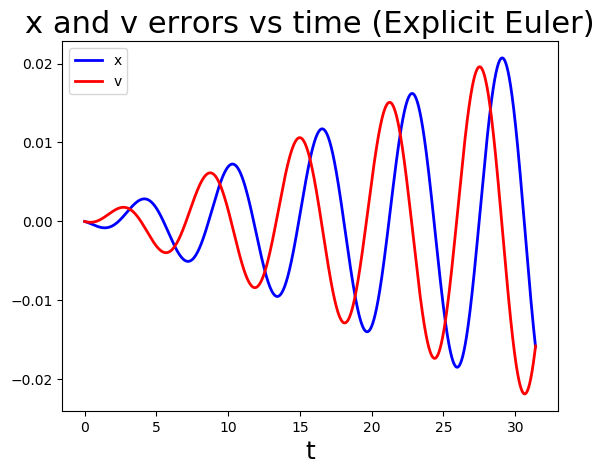
\includegraphics[width = 3in]{Explicit_Errors_X0_1_0_V0_1_0}}
\subfloat[$X_{0}=2$, $V_{0}=1$]{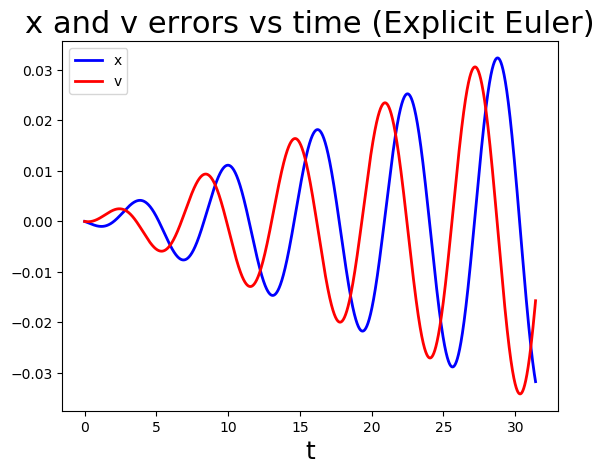
\includegraphics[width = 3in]{Explicit_Errors_X0_2_0_V0_1_0}} 
\caption{Explicit Euler global errors. Regardless of the choice of initial conditions, the errors grow over time.}
\end{figure}

 \begin{figure}[H]
\subfloat[$X_{0}=0$, $V_{0}=1$]{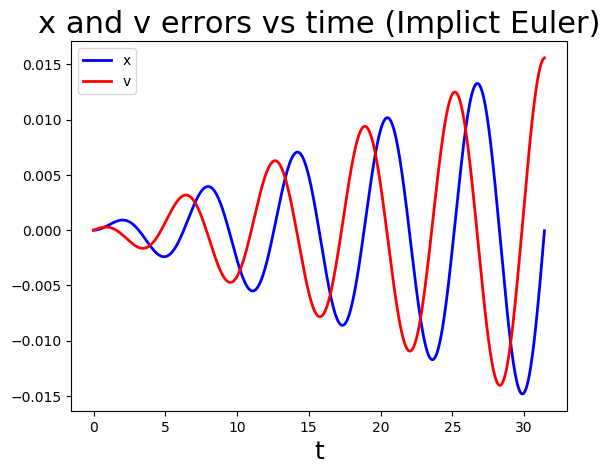
\includegraphics[width = 3in]{Implicit_Errors_X0_0_0_V0_1_0}} 
\subfloat[$X_{0}=1$, $V_{0}=0$]{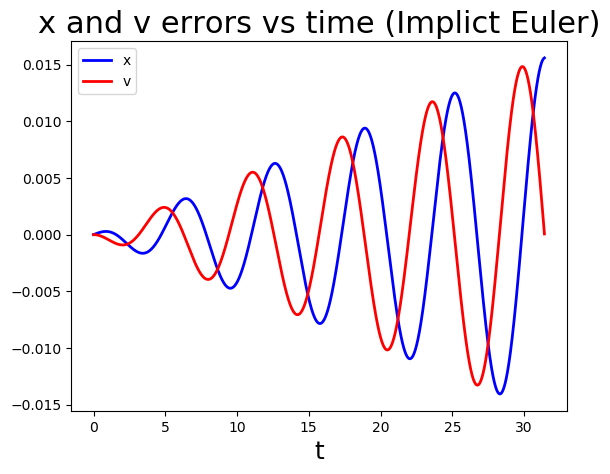
\includegraphics[width = 3in]{Implicit_Errors_X0_1_0_V0_0_0}}\\
\subfloat[$X_{0}=1$, $V_{0}=1$]{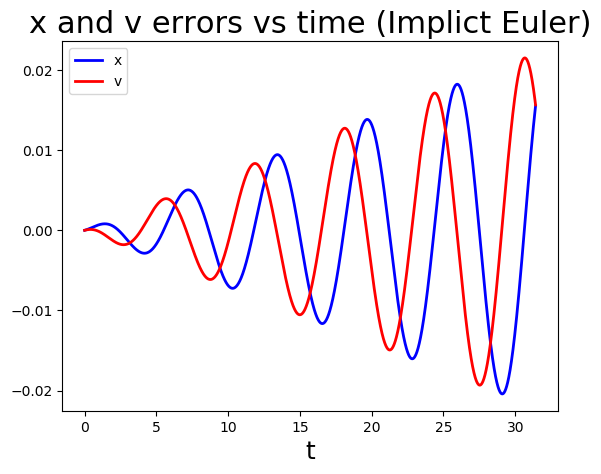
\includegraphics[width = 3in]{Implicit_Errors_X0_1_0_V0_1_0}}
\subfloat[$X_{0}=2$, $V_{0}=1$]{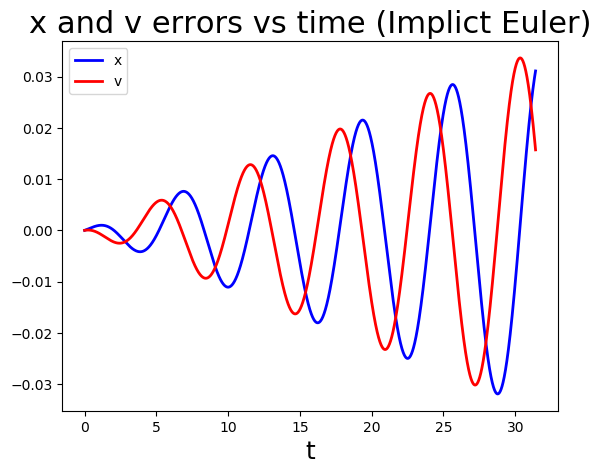
\includegraphics[width = 3in]{Implicit_Errors_X0_2_0_V0_1_0}} 
\caption{Implicit Euler global errors. Notice how they are just the negative of the Explicit ones. This makes sense since we are essentially going "backwards" with this method compared to the explicit method (i.e. using using new values to compute old ones rather than vice versa). }
\end{figure}

\section{Truncation Error}
 \begin{figure}[H]
\subfloat[$X_{0}=0$, $V_{0}=1$]{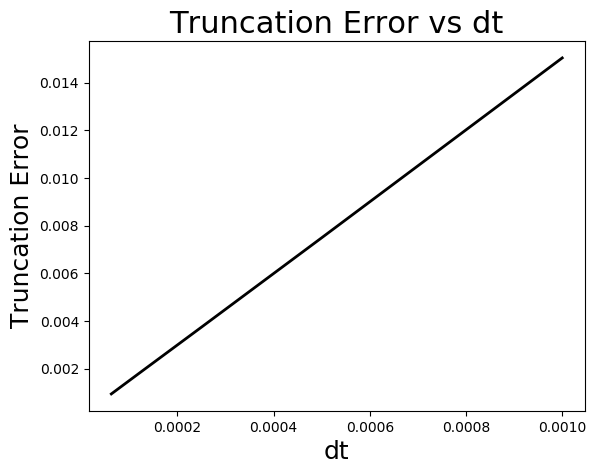
\includegraphics[width = 3in]{Truncation_X0_0_0_V0_1_0}} 
\subfloat[$X_{0}=1$, $V_{0}=0$]{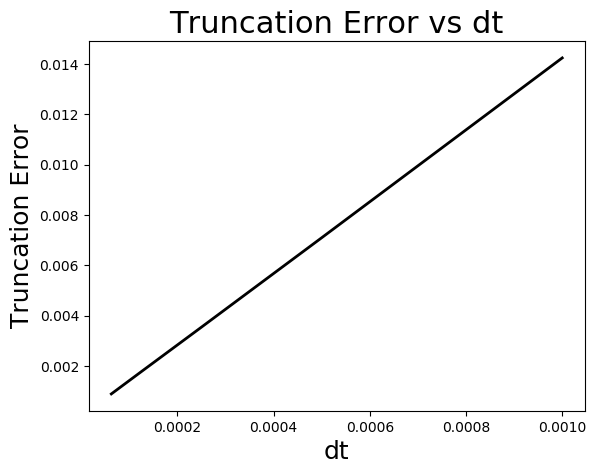
\includegraphics[width = 3in]{Truncation_X0_1_0_V0_0_0}}\\
\subfloat[$X_{0}=1$, $V_{0}=1$]{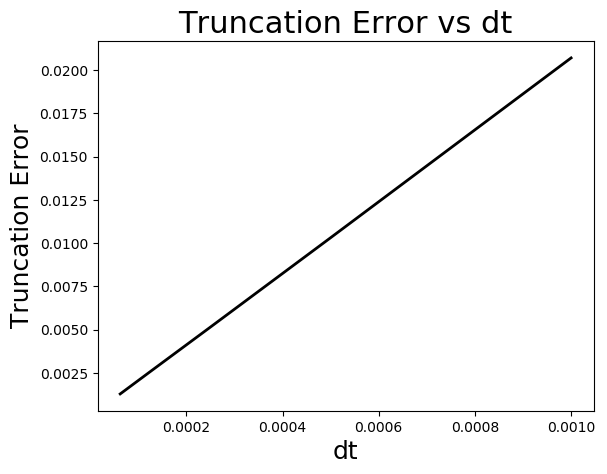
\includegraphics[width = 3in]{Truncation_X0_1_0_V0_1_0}}
\subfloat[$X_{0}=2$, $V_{0}=1$]{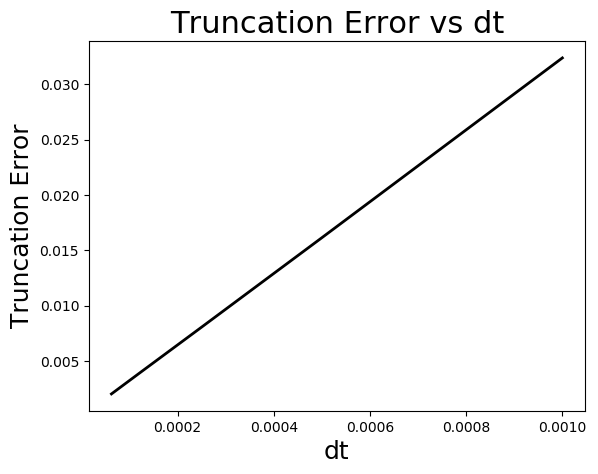
\includegraphics[width = 3in]{Truncation_X0_2_0_V0_1_0}} 
\caption{Truncation error versus step size. For relatively small step sizes, the truncation error is proportional to the step size regardless of initial conditions. It is also independent of the Euler method we choose. This linear relationship between truncation error and step size is also positive as expected, implying that larger steps lead to more error.}
\end{figure}

\section{Total Energy}
 \begin{figure}[H]
\subfloat[$X_{0}=0$, $V_{0}=1$]{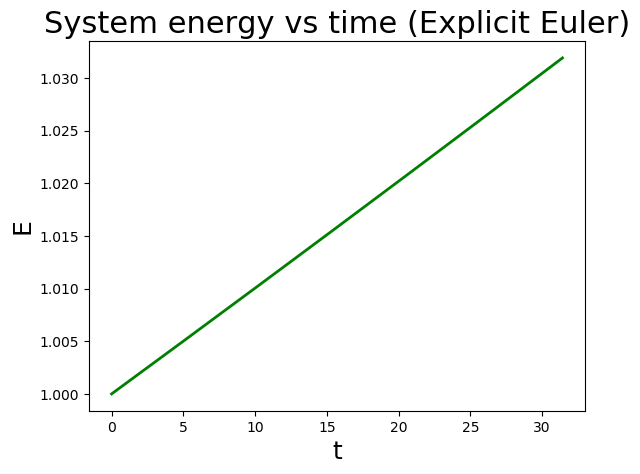
\includegraphics[width = 3in]{Explicit_Energy_X0_0_0_V0_1_0}} 
\subfloat[$X_{0}=1$, $V_{0}=0$]{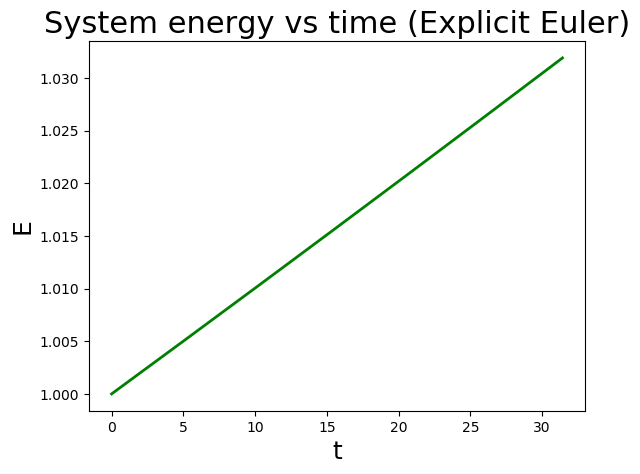
\includegraphics[width = 3in]{Explicit_Energy_X0_1_0_V0_0_0}}\\
\subfloat[$X_{0}=1$, $V_{0}=1$]{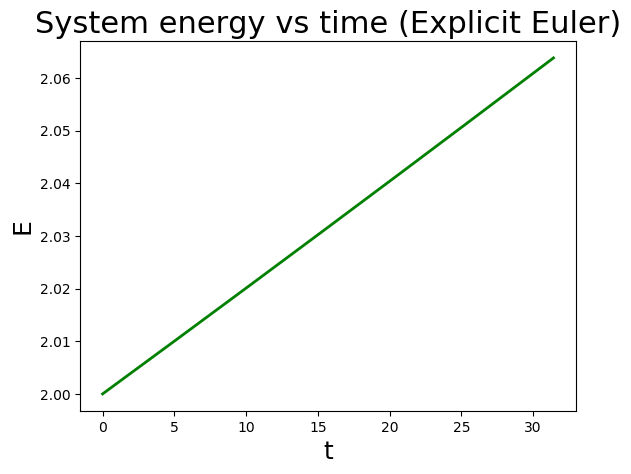
\includegraphics[width = 3in]{Explicit_Energy_X0_1_0_V0_1_0}}
\subfloat[$X_{0}=2$, $V_{0}=1$]{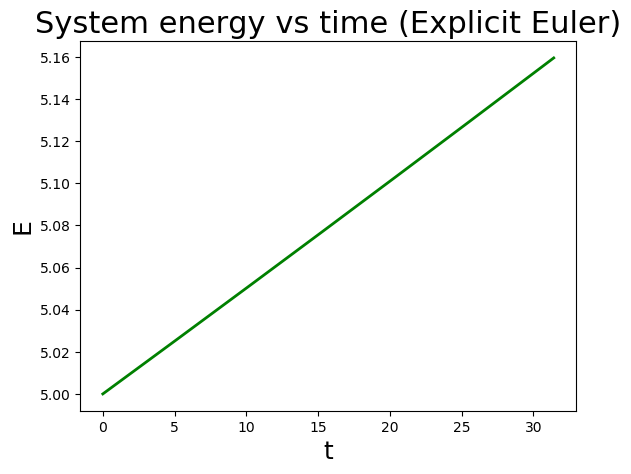
\includegraphics[width = 3in]{Explicit_Energy_X0_2_0_V0_1_0}} 
\caption{Total system energy given by the numerical explicit Euler method.}
\end{figure}

 \begin{figure}[H]
\subfloat[$X_{0}=0$, $V_{0}=1$]{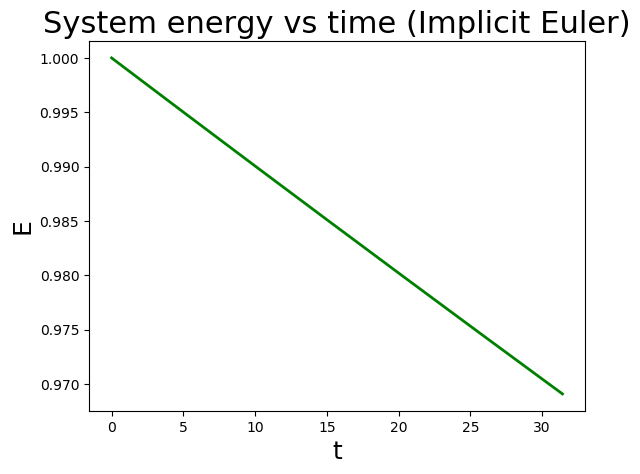
\includegraphics[width = 3in]{Implicit_Energy_X0_0_0_V0_1_0}} 
\subfloat[$X_{0}=1$, $V_{0}=0$]{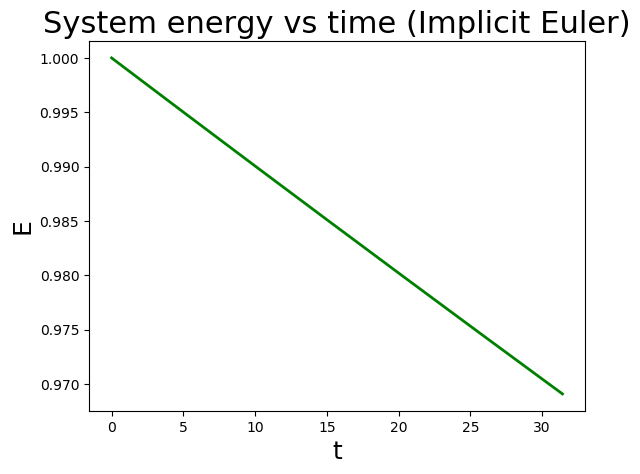
\includegraphics[width = 3in]{Implicit_Energy_X0_1_0_V0_0_0}}\\
\subfloat[$X_{0}=1$, $V_{0}=1$]{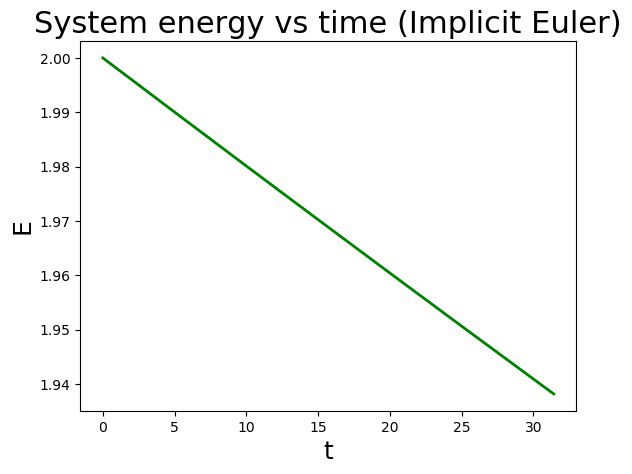
\includegraphics[width = 3in]{Implicit_Energy_X0_1_0_V0_1_0}}
\subfloat[$X_{0}=2$, $V_{0}=1$]{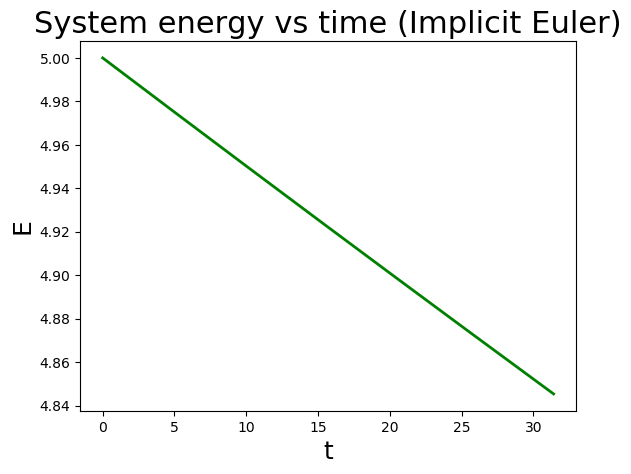
\includegraphics[width = 3in]{Implicit_Energy_X0_2_0_V0_1_0}} 
\caption{Total system energy given by the numerical implicit Euler method.}
\end{figure}

\par Notice how in both cases, the system energy increases over time when it should remain constant. This is because we are adding the squares of position and velocity, which is comparable to adding their amplitudes within a scale factor. However, as the global error plots show, the amplitude of our numerical solutions  is increasing/decreasing (Explicit/Implicit) relative to that of the analytic answers, whose amplitudes remain constant. These changing amplitude of our estimates is why our energy grows or shrinks over time.

 \begin{figure}[H]
\subfloat[$X_{0}=2$, $V_{0}=1$]{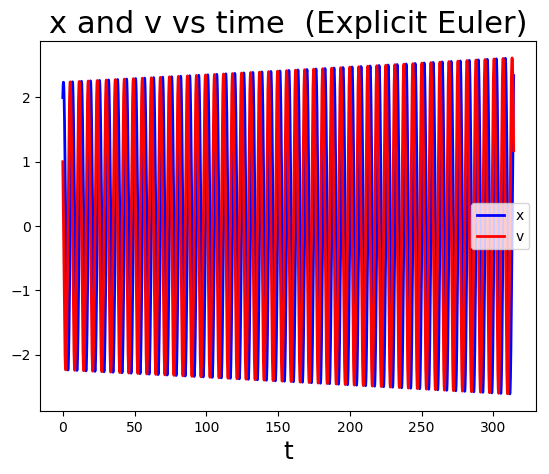
\includegraphics[width = 3in]{long_Explicit_X0_2_0_V0_1_0}} 
\subfloat[$X_{0}=2$, $V_{0}=1$]{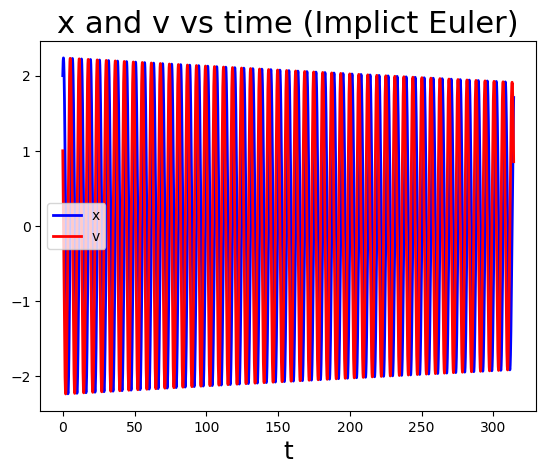
\includegraphics[width = 3in]{long_Implicit_X0_2_0_V0_1_0}}\\
\caption{After many cycles, the explicit solution grows while the implicit one shrinks.}
\end{figure}

\section{Phase Space and Symplectic Integration}

 \begin{figure}[H]
\subfloat[$t=4 \pi$]{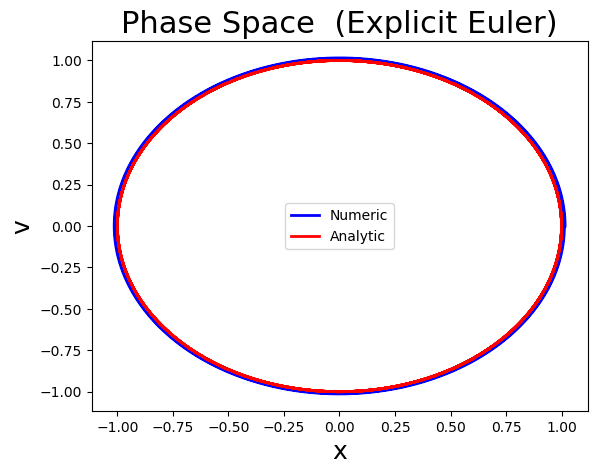
\includegraphics[width = 3in]{Explicit_Phase_X0_1_0_V0_0_0}} 
\subfloat[$t=4 \pi$]{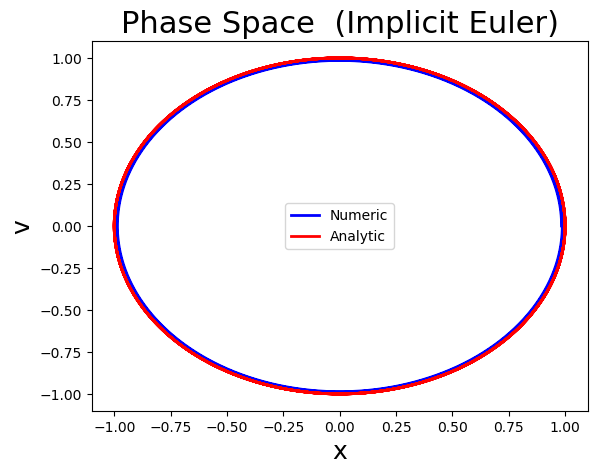
\includegraphics[width = 3in]{Implicit_Phase_X0_1_0_V0_0_0}}\\
\subfloat[$t=100 \pi$]{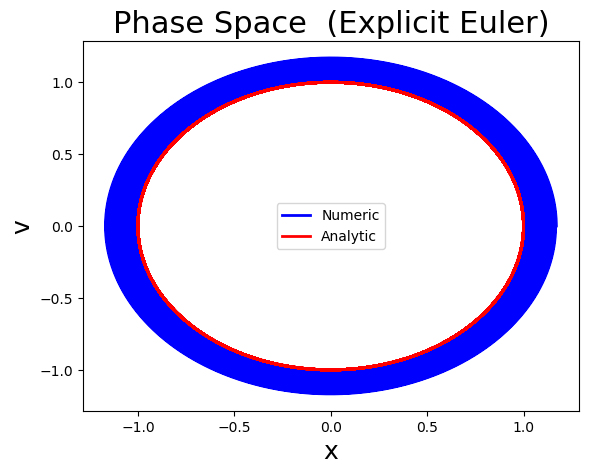
\includegraphics[width = 3in]{long_Explicit_Phase_X0_1_0_V0_0_0}}
\subfloat[$t=100 \pi$]{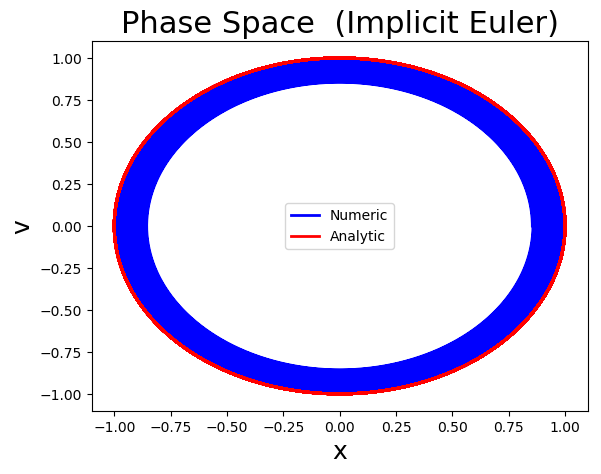
\includegraphics[width = 3in]{long_Implicit_Phase_X0_1_0_V0_0_0}} 
\caption{Phase space plots for both the Explicit and Implicit Euler methods for initial conditions $x_{0}=1$, $v_{0}=0$. As time goes on, error in the system energy calculation does not preserve area in phase space. The area for the Explicit curve increase while the area of the Implicit curve decreases, corresponding to increasing and decreasing system energy respectively.}
\end{figure}


 \begin{figure}[H]
\subfloat[$t=4 \pi$]{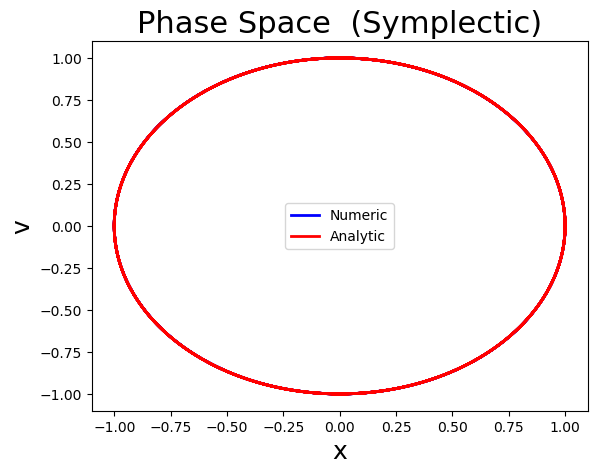
\includegraphics[width = 3in]{Symplectic_Phase_X0_1_0_V0_0_0}} 
\subfloat[$t=100 \pi$]{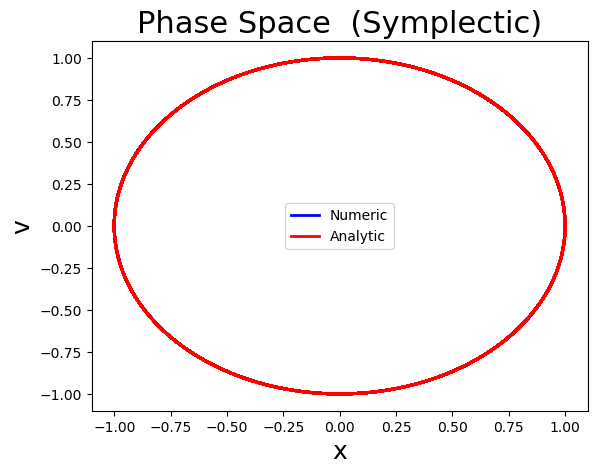
\includegraphics[width = 3in, height = 2.4in]{long_Symplectic_Phase_X0_1_0_V0_0_0}}\\ 
\caption{Phase space plots for both the Symplectic methods for initial conditions $x_{0}=1$, $v_{0}=0$. Regardless of the length of time, this scheme preserves area in phase space.}
\end{figure}

 \begin{figure}[H]
\subfloat[$t=4 \pi$]{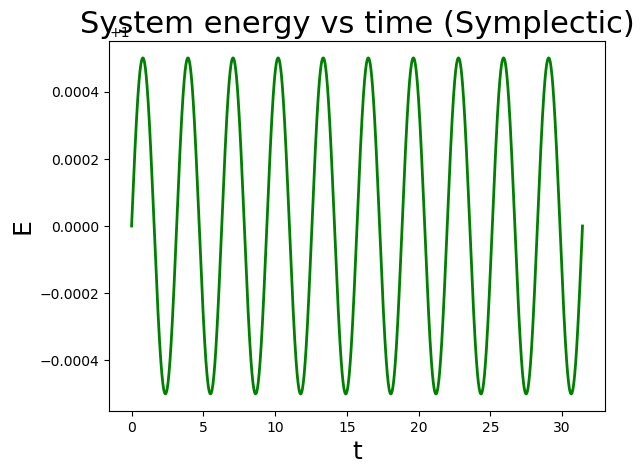
\includegraphics[width = 3in]{Symplectic_Energy_X0_1_0_V0_0_0}} 
\subfloat[$t=100 \pi$]{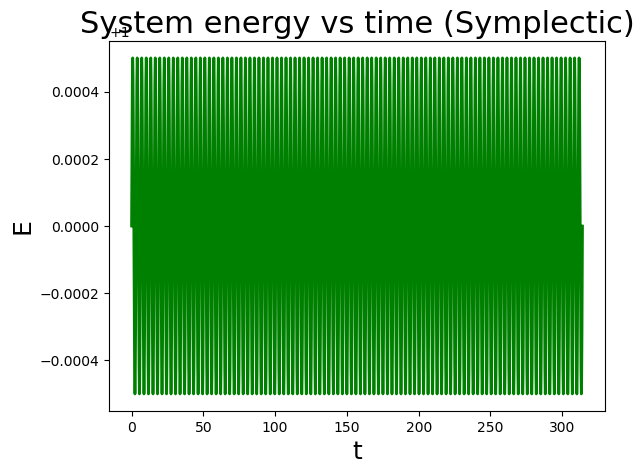
\includegraphics[width = 3in, height = 2.2in]{long_Symplectic_Energy_X0_1_0_V0_0_0}}\\ 
\caption{Plots of offset total system energy over time for the symplectic method. This numeric solution oscillates over time, but on average the energy is constant, reflecting how the radius of the circle in phase space is constant around one cycle.}
\end{figure}

\section{pythoncode}
\verbatiminput{HW3.py}

\section{Git Log}
\input{gitlog.txt}

\end{document}